\documentclass[a4paper,12pt]{article}

\usepackage[utf8]{inputenc}
\usepackage[brazil]{babel}
\usepackage{multicol}
\usepackage{enumitem}
\usepackage[a4paper,margin=1.5cm]{geometry}
\usepackage{array}
\usepackage{graphicx}
\usepackage{xcolor}

\begin{document}
\pagestyle{empty}

% =========================================================
% CABEÇALHO
% =========================================================

\begin{table}[h]
\centering
\renewcommand{\arraystretch}{0.6}

\begin{tabular}{|>{\centering\arraybackslash}m{0.20\textwidth}|>{\centering\arraybackslash}m{0.73\textwidth}|}
\hline


\includegraphics[width=2.8cm]{fpf.png}
&
{
\centering
\vspace{0.2cm}
\textbf{\scriptsize CURSO TÉCNICO EM AUTOMAÇÃO INDUSTRIAL} \\[0.15cm]
\textbf{\small Disciplina: Eletrônica Digital 1} \\[0.15cm]
\textbf{\small AVALIAÇÃO 1}
}

\tabularnewline
\hline
\end{tabular}

\end{table}

\vspace{0.1cm}

% =========================================================
% DADOS DO ALUNO
% =========================================================

\begin{table}[h]
\centering
\renewcommand{\arraystretch}{1.5}

\begin{tabular}{|>{\raggedright\arraybackslash}m{0.70\textwidth}|>{\raggedright\arraybackslash}m{0.23\textwidth}|}
\hline

\textbf{Aluno(a):} & \textbf{Data:} \\
\hline

\textbf{Professor(a):} & \textbf{Nota:} \\
\hline

\end{tabular}

\end{table}

\vspace{0.05cm}

% =========================================================
% INSTRUÇÕES
% =========================================================

\noindent
\begin{minipage}{\textwidth}
\scriptsize
\begin{itemize}[itemsep=0pt, topsep=0pt, parsep=0pt]
    \item Responda a prova com caneta azul ou preta e não use corretivo, do contrário o(a) aluno(a) não terá direito a questionamentos sobre a correção da prova.
    \item Marque a alternativa escolhida com preenchimento no Cartão-resposta.
    \item Proibido, durante a prova, o uso de telefone celular e/ou aparelhos eletroeletrônicos, empréstimos de materiais, conversas paralelas, nenhum tipo de consulta e sair da sala de aula sem autorização.
    \item O(a) aluno(a) receberá nota 0,0 (Zero), caso seja surpreendido em comunicação com outro aluno de forma verbal ou escrita.
\end{itemize}
\end{minipage}

\vspace{0.5cm}
\noindent\rule{\textwidth}{1pt}

% =========================================================
% PROVA
% =========================================================

\begin{multicols}{2}
\raggedcolumns

\textbf{Cartão-resposta:}

\vspace{0.2cm}

\begin{tabular}{|c|c|c|c|c|c|}
\hline
\textbf{Questões} & A & B & C & D & E \\
\hline
01 & O & O & O & O & O \\
\hline
02 & O & O & O & O & O \\
\hline
03 & O & O & O & O & O \\
\hline
04 & O & O & O & O & O \\
\hline
05 & O & O & O & O & O \\
\hline
06 & O & O & O & O & O \\
\hline
07 & O & O & O & O & O \\
\hline
08 & O & O & O & O & O \\
\hline
09 & O & O & O & O & O \\
\hline
10 & O & O & O & O & O \\
\hline
\end{tabular}

\vspace{0.7cm}

\begin{enumerate}[leftmargin=*]

% =========================================================
% QUESTÃO 1
% =========================================================

\item \textbf{(0,5 pontos)} Um sensor está conectado a um conversor ADC.
A tensão do sensor muda um pouco, mas o valor digital do ADC continua o mesmo.
Por que isso pode acontecer?

\begin{enumerate}[label=(\Alph*)]
    \item Porque o ADC está com defeito.
    \item Porque o ADC agrupa valores de tensão próximos em um mesmo valor digital.
    \item Porque o ADC não consegue medir tensão.
    \item Porque o ADC transforma qualquer tensão no mesmo valor digital.
    \item Porque o ADC sempre ignora pequenas tensões de entrada.
\end{enumerate}

\vspace{0.2cm}

% =========================================================
% QUESTÃO 2
% =========================================================

\item \textbf{(0,5 pontos)} Um sinal digital apresenta, em sequência, os seguintes níveis lógicos:

\[
0 \rightarrow 0 \rightarrow 1 \rightarrow 1 \rightarrow 0
\]

Qual alternativa descreve corretamente o comportamento desse sinal?

\begin{enumerate}[label=(\Alph*)]
    \item Ocorreram quatro transições, pois foram observados cinco níveis.
    \item Ocorreram duas transições: uma de subida e uma de descida.
    \item Ocorreu apenas uma transição, quando o sinal passou de $0$ para $1$.
    \item Ocorreram três transições, pois toda repetição de um nível lógico representa uma nova transição.
    \item Não ocorreu nenhuma transição, pois o sinal começou e terminou em nível lógico $0$.
\end{enumerate}

\vspace{0.2cm}

% =========================================================
% QUESTÃO 3
% =========================================================

\item \textbf{(0,5 pontos)} Um CLP possui um registrador de 2 bytes.
Considerando que o registrador armazena apenas números inteiros sem sinal,
qual é o maior valor decimal que pode ser armazenado nele?

\begin{enumerate}[label=(\Alph*)]
    \item $255_{10}$
    \item $1023_{10}$
    \item $32767_{10}$
    \item $65535_{10}$
    \item $65536_{10}$
\end{enumerate}

\vspace{0.2cm}

% =========================================================
% QUESTÃO 4
% =========================================================

\item \textbf{(0,5 pontos)} Um sistema digital precisa representar o número
decimal $45_{10}$ em binário. Qual das alternativas apresenta a conversão correta?

\begin{enumerate}[label=(\Alph*)]
    \item $101011_2$
    \item $101101_2$
    \item $110101_2$
    \item $101110_2$
    \item $110011_2$
\end{enumerate}
% =========================================================
% QUESTÃO 5
% =========================================================

\item \textbf{(0,5 pontos)} Qual é o valor em decimal correspondente ao número binário $110101_2$?

\begin{enumerate}[label=(\Alph*)]
    \item $51_{10}$
    \item $53_{10}$
    \item $55_{10}$
    \item $57_{10}$
    \item $61_{10}$
\end{enumerate}

% =========================================================
% QUESTÃO 6
% =========================================================

\item \textbf{(0,5 pontos)} Considere os dois números binários:

\[
A = 101101_2
\]

\[
B = 110011_2
\]

Ao realizar a operação lógica \textbf{OU Exclusivo (XOR)} bit a bit entre
$A$ e $B$, qual será o resultado?

\begin{enumerate}[label=(\Alph*)]
    \item $011110_2$
    \item $111111_2$
    \item $100001_2$
    \item $010010_2$
    \item $101110_2$
\end{enumerate}

\vspace{0.2cm}

% =========================================================
% QUESTÃO 7
% =========================================================

\item \textbf{(0,5 pontos)} Considere os dois números binários:

\[
A = 101101_2
\]

\[
B = 110011_2
\]

Ao realizar a operação lógica \textbf{AND} bit a bit entre $A$ e $B$,
qual será o resultado?

\begin{enumerate}[label=(\Alph*)]
    \item $100001_2$
    \item $111111_2$
    \item $011110_2$
    \item $110101_2$
    \item $101001_2$
\end{enumerate}

\vspace{0.2cm}

% =========================================================
% QUESTÃO 8
% =========================================================

\item \textbf{(0,5 pontos)} Considere o número binário de 8 bits:

\[
A = 10110010_2
\]

Ao realizar a operação lógica \textbf{NOT} sobre todos os bits de $A$,
qual será o resultado?

\begin{enumerate}[label=(\Alph*)]
    \item $01001101_2$
    \item $10110011_2$
    \item $01011101_2$
    \item $11001101_2$
    \item $00110010_2$
\end{enumerate}

\vspace{0.2cm}

% =========================================================
% QUESTÃO 9
% =========================================================

\item \textbf{(0,5 pontos)} Considere os dois números binários:

\[
A = 101101_2
\]

\[
B = 110011_2
\]

Ao realizar a operação lógica \textbf{OR} bit a bit entre $A$ e $B$,
qual será o resultado?

\begin{enumerate}[label=(\Alph*)]
    \item $100001_2$
    \item $111111_2$
    \item $011110_2$
    \item $110101_2$
    \item $101111_2$
\end{enumerate}

% =========================================================
% QUESTÃO 10
% =========================================================

\item \textbf{(0,5 pontos)} Considere o seguinte circuito:


\begin{center}
    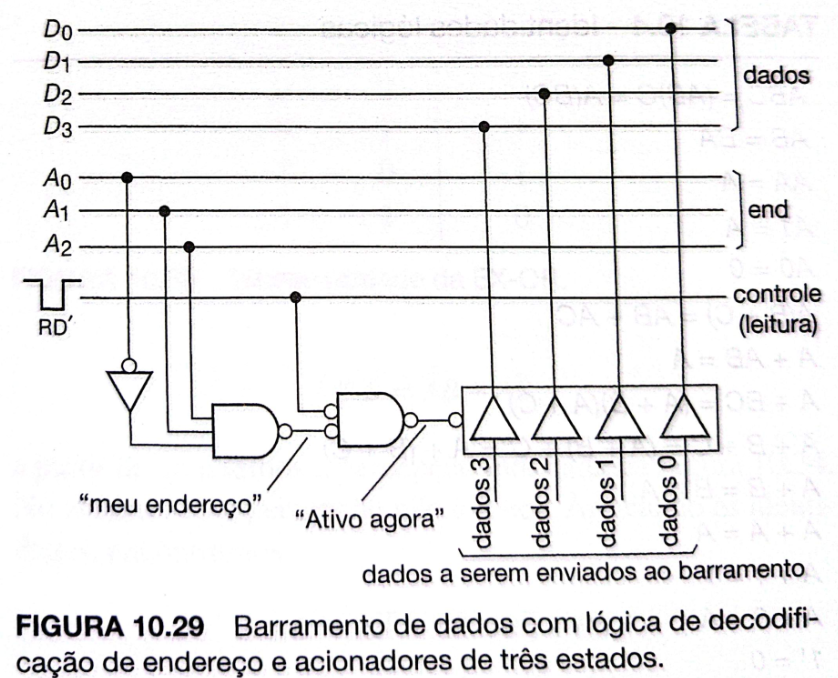
\includegraphics[width=0.75\columnwidth]{figura.png}
\end{center}

Qual a equação boleana que descreve o circuito até consta "ativo agora"?

\begin{enumerate}[label=(\Alph*)]
    \item $\overline{A_0} \cdot A_1 \cdot A_2 \cdot RD'$
    \item $A_0 \cdot \overline{A_1} \cdot A_2 \cdot RD'$
    \item $A_0 \cdot A_1 \cdot \overline{A_2} \cdot RD'$
    \item $A_0 \cdot A_1 \cdot A_2 \cdot \overline{RD'}$
    \item $\overline{A_0 \cdot A_1 \cdot A_2 \cdot RD'}$
\end{enumerate}


\end{enumerate}

\end{multicols}

\vfill

\end{document}